\documentclass[border=10pt]{standalone}

\usepackage{tikz}
\usepackage{tikzsymbols}
\usetikzlibrary{calc,patterns,shapes.geometric}

\def\centerarc[#1](#2)(#3:#4:#5){\draw[#1] ($(#2)+({#5*cos(#3)},{#5*sin(#3)})$) arc (#3:#4:#5);}

\begin{document}
	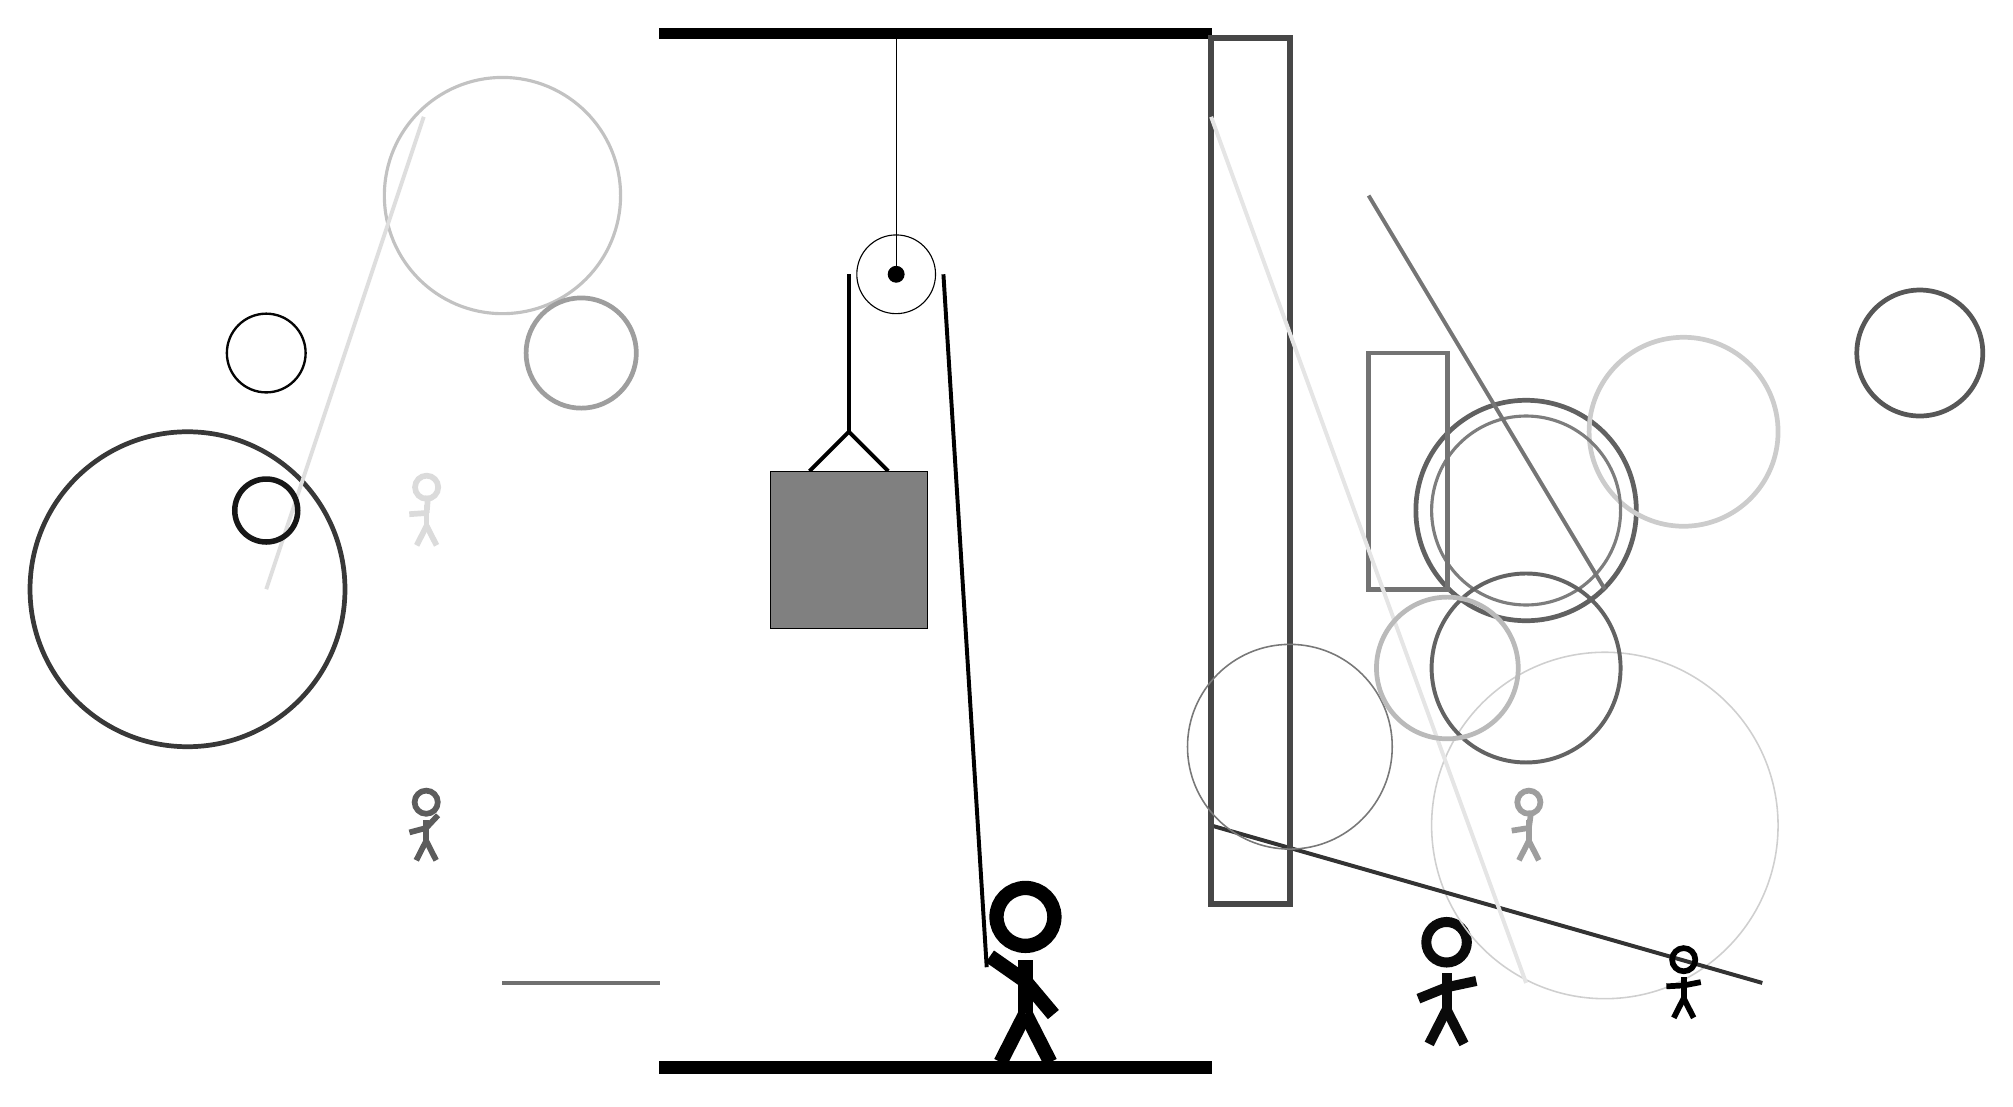
\begin{tikzpicture}
		%%%%% START %%%%%
		
		\draw[fill=black] (-2, 10) rectangle (5, 10.125);
		
		\draw (1, 7) circle (0.5);
		\draw[fill=black] (1, 7) circle (0.1);
		\draw (1, 10) -- (1, 7);
		
		\draw[line width=0.5mm] (-0.1, 4.5) -- (0.4, 5.0) -- (0.9, 4.5);
		\draw[fill=black!50] (-0.6, 4.5) rectangle (1.4, 2.5);
		
		\draw[line width=0.5mm] (0.4, 7) -- (0.4, 5.0);
		\centerarc[line width=0.5mm](1, 7)(0:180:0.6);
		\draw[line width=0.5mm](1.6, 7) -- (2.15, -1.8);
		
		\node at (2.6, -1.9) {\Strichmaxerl[10][-35][-50]};
		
		\node[line width=0.7mm, color=black!96] at (8, -2) {\Strichmaxerl[7][22][12]};
		
		\draw [line width=0.6mm, color=black!78](-8, 3) circle (2.0);
		\draw [line width=0.6mm, color=black!62](9, 4) circle (1.4);
		\draw [line width=0.4mm, color=black!24](-4, 8) circle (1.5);
		
		\draw [line width=0.6mm, color=black!20](11, 5) circle (1.2);
		\draw [line width=0.4mm, color=black!51](9, 4) circle (1.2);
		\draw[line width=0.5mm, color=black!56](-4, -2) -- (-2, -2);
		\draw [line width=0.2mm, color=black!19](10, 0) circle (2.2);
		\node[line width=0.6mm, color=black!14] at (-5, 4) {\Strichmaxerl[4][4][85]};
		\draw[line width=0.5mm, color=black!80](5, 0) -- (12, -2);
		\draw[line width=0.6mm, color=black!98] (7, 4) rectangle (7, 3);
		
		\draw[line width=0.5mm, color=black!13](-5, 9) -- (-7, 3);
		\draw [line width=0.6mm, color=black!38](-3, 6) circle (0.7);
		
		\draw[line width=0.6mm, color=black!55] (7, 3) rectangle (8, 6);
		\draw [line width=0.3mm, color=black!98](-7, 6) circle (0.5);
		\draw[line width=0.7mm, color=black!72] (6, 10) rectangle (5, -1);
		
		\node[line width=0.6mm, color=black!64] at (-5, 0) {\Strichmaxerl[4][15][47]};
		\node[line width=0.2mm, color=black!100] at (11, -2) {\Strichmaxerl[4][3][11]};
		\draw [line width=0.2mm, color=black!53](6, 1) circle (1.3);
		\draw [line width=0.5mm, color=black!61](9, 2) circle (1.2);
		\draw[line width=0.5mm, color=black!10](9, -2) -- (5, 9);
		\draw [line width=0.7mm, color=black!91](-7, 4) circle (0.4);
		\draw [line width=0.6mm, color=black!66](14, 6) circle (0.8);
		\draw [line width=0.6mm, color=black!27](8, 2) circle (0.9);
		\draw[line width=0.5mm, color=black!54](7, 8) -- (10, 3);
		
		\node[line width=0.3mm, color=black!38] at (9, 0) {\Strichmaxerl[4][9][82]};
		
		
		\draw[fill=black] (-2, -3) rectangle (5, -3.15);
		
		%%%%% END %%%%%
	\end{tikzpicture}
\end{document}